\chapter{\MakeUppercase{Resultados e discussão}}\label{sec:resultados-discussao}

Os resultados relacionam a caracterização das instâncias, o povoamento do
mapa fixo e as trajetórias do IBS à comparação de seis abordagens exatas
e heurísticas quanto à qualidade das soluções e ao custo computacional.
A coleção final reúne 74 instâncias e 3.936 execuções comparativas;
as trajetórias complementares provêm de outras 190 execuções nas adições.
As médias utilizam exclusivamente o experimento comparativo, com BKV e
agregação definidos na Seção~\ref{sec:met-analise}. As tabelas detalhadas
por instância e os registros de auditoria foram preservados nos arquivos
do projeto.

\section{Caracterização das instâncias e dos atributos}\label{sec:res-caracterizacao}

A base original contém 16 instâncias clássicas e 39 do gerador associado
a \citeonline{DelazeriRitt2026}. Dessas 55, 49 pertencem a \textit{Small}
ou \textit{Medium}; entre as 19 adições, 15 são \textit{Large} ou
\textit{Huge}. A Tabela~\ref{tab:res-perfil} mostra que a expansão também
alterou recursos, liberações e tempos de propagação. Essas propriedades
variam conjuntamente e não permitem isolar a causa das diferenças de
desempenho observadas adiante.

\begin{table}[!htbp]
\centering
\caption{Características das coleções original e gerada.}
\label{tab:res-perfil}
\begin{singlespace}
\normalsize
\setlength{\tabcolsep}{5pt}
\renewcommand{\arraystretch}{1.15}
\begin{tabular}{lrr}
\hline\hline
\textbf{Atributo} & \textbf{55 originais} & \textbf{19 geradas} \\
\hline
Vértices & 900 [329; 900] & 1600 [1600; 6400] \\
Recursos totais & 30 [18; 30] & 40 [20; 40] \\
Recursos por liberação & 3,0 [3,0; 3,0] & 2,0 [1,0; 2,0] \\
Primeira liberação/$H$ & 0,101 [0,081; 0,143] & 0,253 [0,152; 0,275] \\
Última liberação/$H$ & 0,691 [0,571; 0,698] & 0,749 [0,729; 0,766] \\
Atraso/$H$ & 1,000 [0,607; 1,000] & 0,500 [0,333; 1,000] \\
CV dos tempos dos arcos & 0,436 [0,436; 0,476] & 0,577 [0,559; 0,596] \\
\hline\hline
\end{tabular}
\par\smallskip
{\small Nota: mediana [primeiro quartil; terceiro quartil]. As razões temporais e o coeficiente de variação (CV) são adimensionais.\par}
{\fonte{elaboração própria a partir dos dados experimentais.}}
\end{singlespace}
\end{table}


As 55 originais compartilham 20 grafos direcionados de propagação distintos, enquanto
as adições introduzem outros 19. Assim, as 74 instâncias representam
39 grafos combinados a configurações de recursos e liberações; a contagem
de arquivos não equivale a observações amostradas independentemente.
Na exploração inicial, a PCA preservou 74,18\% da variância dos atributos
originais em duas dimensões, resultado de compressão que não mede
capacidade preditiva.

Nas florestas aleatórias dessa exploração inicial, os atributos de maior
importância para classificar o melhor método foram recursos por liberação,
recursos totais e média de chegadas entre liberações. Para estimar a menor
mediana de \textit{gap}, destacaram-se recursos por liberação, média de
chegadas entre liberações e perímetro médio nas liberações. Os dois
resultados destacam a disponibilidade de recursos e o avanço da propagação
entre suas liberações. São importâncias obtidas nos ajustes históricos,
não uma avaliação preditiva dos modelos ISA finais.

A auditoria reteve 73 dos 136 candidatos topológicos, conforme os critérios
da Seção~\ref{sec:met-topologia}. Os oito resumos de agrupamento dirigido
foram constantes, ilustrando que medidas genéricas de redes podem não
discriminar os grafos deste domínio. A retirada de duplicatas e atributos
HITS instáveis evitou incorporar redundância exata ou variação numérica
como características do problema.

\section{Geração orientada e cobertura do mapa de referência}\label{sec:res-geracao}

As três sementes produziram 36 buscas e 72.000 avaliações, resultando em
19 instâncias aceitas e distintas: sete, seis e seis por semente.
Duas buscas foram classificadas como \textit{hit}, 17 como
\textit{improved} e 17 como \textit{missed}; estas incluem quatro finalistas
que se aproximaram do alvo, mas ficaram fora do domínio após recomputação
exata. A aceitação em 52,78\% das buscas demonstra viabilidade do povoamento,
embora a maioria das aproximações não tenha alcançado o critério mais
restrito de \textit{hit}.

A Figura~\ref{fig:res-geracao} mostra as adições no mapa histórico fixo.
Como na proposta de \citeonline{SmithMilesBowly2015}, a cobertura é avaliada
reutilizando atributos, transformações e projeção. Os modelos ISA finais,
reajustados com os novos desempenhos, possuem outra geometria.

\begin{figure}[!htbp]
\centering
\caption{Posição das instâncias aceitas no mapa fixo de geração.}
\label{fig:res-geracao}
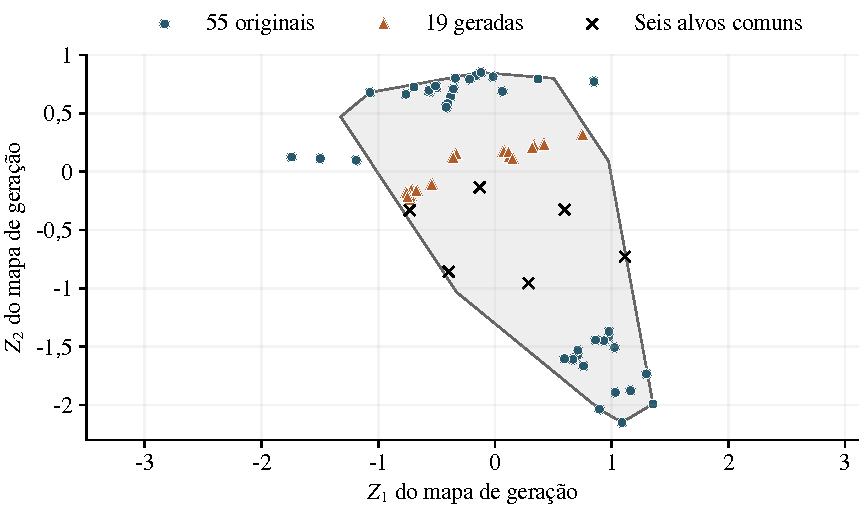
\includegraphics[width=\textwidth]{imgs/resultados/geracao_mapa_fixo.pdf}
\begin{singlespace}
{\small Legenda: círculos indicam as 55 originais; triângulos, as 19 adições;
cruzes, os seis alvos comuns às três sementes no primeiro lote de geração.
A região sombreada é o domínio interno. Os alvos adaptativos do segundo
lote não estão representados.\par}
{\fonte{elaboração própria a partir das coordenadas do experimento de geração.}}
\end{singlespace}
\end{figure}

A Tabela~\ref{tab:res-cobertura} compara as sequências e sua união sobre
o mesmo domínio e os mesmos 10.000 pontos Sobol. Na união, a distância
máxima diminuiu 20,92\%, a média diminuiu 36,27\% e a ocupação passou de
15\% para 20\%. Entretanto, 52,54\% dos pontos continuaram acima do limiar
de subcobertura, e a união não superou a melhor semente na distância
máxima. Houve preenchimento parcial, com lacunas remanescentes.

\begin{table}[!htbp]
\centering
\caption{Cobertura antes e depois das adições no mapa de geração fixo.}
\label{tab:res-cobertura}
\begin{singlespace}
\normalsize
\setlength{\tabcolsep}{5pt}
\renewcommand{\arraystretch}{1.15}
\begin{tabular}{lrrrrr}
\hline\hline
\textbf{Coleção} & \textbf{Adições} & \textbf{\shortstack{Distância\\máxima}} & \textbf{\shortstack{Distância\\média}} & \textbf{\shortstack{Subcobertura\\(\%)}} & \textbf{\shortstack{Ocupação\\(\%)}} \\
\hline
Base original & 0 & 1,2401 & 0,5284 & 71,70 & 15 \\
20260612 & 7 & 0,9875 & 0,3426 & 54,29 & 19 \\
104729 & 6 & 0,9853 & 0,3615 & 57,44 & 18 \\
1299709 & 6 & 0,9807 & 0,3640 & 59,86 & 18 \\
União das 19 & 19 & 0,9807 & 0,3368 & 52,54 & 20 \\
\hline\hline
\end{tabular}
\par\smallskip
{\small Nota: mesmas transformações, mesmo domínio interno e mesmos 10.000 pontos Sobol em todas as linhas. A ocupação usa uma grade $10\times10$. A linha da união foi recalculada com as coordenadas das 19 aceitações, sem repetir a geração.\par}
{\fonte{elaboração própria a partir dos dados experimentais.}}
\end{singlespace}
\end{table}


O resultado demonstra maior cobertura dessa representação, não de todo
o conjunto de instâncias possíveis do WSP. A ausência de geração aleatória
sob igual orçamento também impede estimar a vantagem da orientação por ISA.

\section{Desempenho dos métodos na coleção ampliada}\label{sec:res-benchmark}

\subsection{Resultados gerais e diferenças entre coleções}

A Tabela~\ref{tab:res-desempenho} resume as 656 execuções por método,
com peso igual por instância. O IBS, adotado como método de referência,
apresentou o menor \textit{gap} médio
global, 3,49\%, e a melhor média em 44 casos, incluindo 37 vitórias
exclusivas. MIP teve \textit{gap} de 15,06\%, mas posição média próxima
à do IBS: frequência das colocações e magnitude das perdas são aspectos
diferentes da comparação.

\begin{table}[!htbp]
\centering
\caption{Desempenho dos seis métodos por coleção.}
\label{tab:res-desempenho}
\begin{singlespace}
\normalsize
\setlength{\tabcolsep}{5pt}
\renewcommand{\arraystretch}{1.15}
\begin{tabular}{lrrrrrr}
\hline\hline
\textbf{Método} & \textbf{\shortstack{\textit{Gap} 55\\(\%)}} & \textbf{\shortstack{\textit{Gap} 19\\(\%)}} & \textbf{\shortstack{\textit{Gap} 74\\(\%)}} & \textbf{\shortstack{Posição\\média}} & \textbf{\shortstack{Melhor\\média}} & \textbf{\shortstack{Melhor média\\exclusiva}} \\
\hline
IBS & 2,65 & 5,92 & 3,49 & 2,07 & 44 & 37 \\
MIP & 18,52 & 5,04 & 15,06 & 2,16 & 11 & 6 \\
CUTH & 29,39 & 3,23 & 22,67 & 2,80 & 20 & 20 \\
LBBD & 38,11 & 9,67 & 30,81 & 4,39 & 11 & 4 \\
ILS & 39,57 & 10,03 & 31,98 & 5,32 & 1 & 0 \\
RS & 43,75 & 9,05 & 34,84 & 4,26 & 0 & 0 \\
\hline\hline
\end{tabular}
\par\smallskip
{\small Nota: \textit{gaps} médios com peso igual por instância. As duas falhas ILS permanecem na análise com a solução viável sem recursos. A coluna melhor média inclui empates; a última coluna conta somente vitórias exclusivas.\par}
{\fonte{elaboração própria a partir dos dados experimentais.}}
\end{singlespace}
\end{table}


O IBS liderou a base original com \textit{gap} médio de 2,65\%, em
consonância com o desempenho favorável relatado por
\citeonline{DelazeriRitt2024,DelazeriRitt2026}, embora os protocolos não
sejam idênticos. Nas adições, CUTH obteve a menor média, 3,23\%, e liderou
15 casos; IBS e MIP lideraram dois cada. A Figura~\ref{fig:res-ibs-cuth}
evidencia esse contraste. A ampliação revelou um regime favorável à CUTH
que a média da coleção original representava pouco.

\begin{figure}[!htbp]
\centering
\caption{Comparação dos \textit{gaps} médios do IBS e de CUTH por instância.}
\label{fig:res-ibs-cuth}
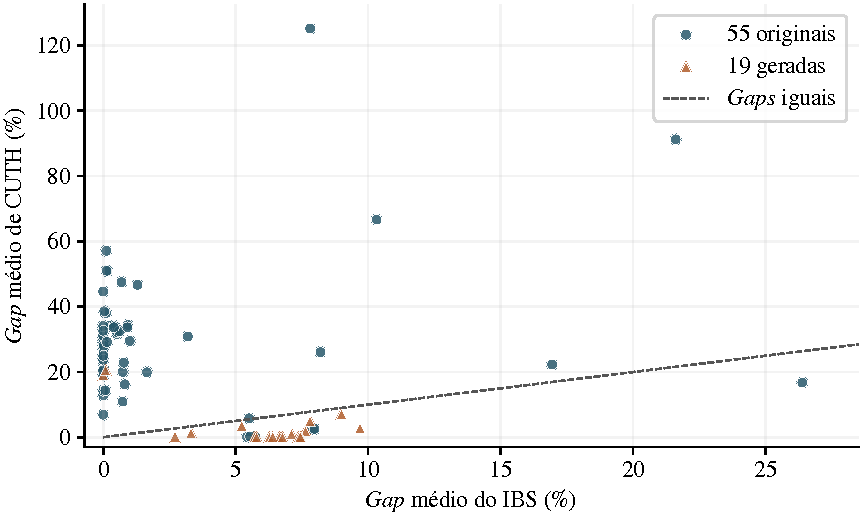
\includegraphics[width=\textwidth]{imgs/resultados/ibs_cuth_instancias.pdf}
\begin{singlespace}
{\small Legenda: cada ponto representa uma instância. Abaixo da igualdade,
CUTH tem menor \textit{gap}; acima, IBS.\par}
{\fonte{elaboração própria a partir dos objetivos reavaliados do experimento.}}
\end{singlespace}
\end{figure}

\subsection{Tamanho, origem e escala dos \textit{gaps}}

IBS apresentou o menor \textit{gap} médio em \textit{Small},
\textit{Medium} e \textit{Large}, e CUTH, em \textit{Huge}
(Tabela~\ref{tab:res-classes}). Essa última classe contém nove adições e
três originais: o \textit{gap} médio de CUTH foi aproximadamente 0,00249\%
nas primeiras e 9,50\% nas últimas. Portanto, o porte não explica sozinho
sua vantagem. Tampouco houve domínio uniforme nas adições: em
\textit{Large}-\texttt{027de052}, CUTH teve 19,03\%, enquanto IBS teve 0,00\%.
Nas adições, CUTH apresentou a menor média nas nove \textit{Huge},
em três das seis \textit{Large} e nas três \textit{Medium}; a única
\textit{Small} foi liderada por MIP. Assim, suas 15 lideranças se
distribuíram por três classes de tamanho.

\begin{table}[!htbp]
\centering
\caption{\textit{Gap} médio por classe de tamanho na coleção de 74 instâncias.}
\label{tab:res-classes}
\begin{singlespace}
\normalsize
\setlength{\tabcolsep}{5pt}
\renewcommand{\arraystretch}{1.15}
\begin{tabular}{lrrrr}
\hline\hline
\textbf{Método} & \textbf{\shortstack{\textit{Small}\\($n=20$)}} & \textbf{\shortstack{\textit{Medium}\\($n=33$)}} & \textbf{\shortstack{\textit{Large}\\($n=9$)}} & \textbf{\shortstack{\textit{Huge}\\($n=12$)}} \\
\hline
IBS & 0,73 & 3,43 & 5,38 & 6,81 \\
MIP & 3,47 & 25,81 & 11,79 & 7,27 \\
CUTH & 23,83 & 31,78 & 13,78 & 2,38 \\
LBBD & 8,01 & 54,73 & 22,46 & 9,31 \\
ILS & 9,49 & 56,18 & 23,29 & 9,42 \\
RS & 29,25 & 51,28 & 21,12 & 9,21 \\
\hline\hline
\end{tabular}
\par\smallskip
{\small Nota: valores em porcentagem, com peso igual por instância. Cada classe contém instâncias originais e geradas.\par}
{\fonte{elaboração própria a partir dos dados experimentais.}}
\end{singlespace}
\end{table}


A escala do BKV exige cautela. Nas nove \textit{Huge} geradas, a melhor
perda observada corresponde a 92,84\%--94,55\% dos 6.400 vértices.
A solução sem recursos já apresenta \textit{gap} médio de 6,80\% nesses
casos, apesar da queima total antes do horizonte. Na coleção original,
seu \textit{gap} médio é 51,12\%; nas adições, 10,10\%. Logo, percentuais
pequenos não demonstram perdas absolutas pequenas nem dificuldade
uniformemente baixa. A solução sem recursos serve aqui à interpretação
da escala e não integra o ranking como um sétimo método.

\subsection{Comparações pareadas}

Além da média global, comparou-se a frequência com que cada método
superou outro nas 74 instâncias. Em cada comparação, considerou-se vencedor
o método com menor \textit{gap} médio nas repetições daquela instância;
os empates foram registrados separadamente. Essa contagem distingue vencer
em muitas instâncias de obter uma grande vantagem em poucas delas.

Aplicou-se o teste de sinal para avaliar o desequilíbrio entre vitórias
e derrotas, excluindo os empates. Como os seis métodos formam 15 pares,
os valores de $p$ receberam a correção de Holm para controlar o risco de
identificar diferenças indevidamente ao realizar múltiplos testes.
Adotou-se o limiar de 0,05: resultados com $p$ ajustado menor ou igual
a esse valor foram considerados estatisticamente significativos.

O IBS apresentou menor média que CUTH em 51 instâncias, enquanto CUTH
venceu nas outras 23. O $p$ ajustado de aproximadamente 0,006065 ficou
abaixo do limiar adotado, indicando uma vantagem estatisticamente
significativa do IBS na frequência de vitórias. Contra MIP, o IBS venceu
42 vezes, empatou cinco e perdeu 27. Nesse caso, o $p$ ajustado de
0,182373 ficou acima de 0,05: o placar favoreceu IBS, mas a evidência foi
insuficiente para concluir uma diferença estatisticamente significativa.
Esse resultado também não demonstra equivalência entre os dois métodos.

A frequência de vitórias deve ser interpretada junto da magnitude dos
\textit{gaps}. A RS, utilizada como linha de base, superou ILS em 58
instâncias e perdeu em 16; contra
LBBD, venceu em 50 e perdeu em 24. Ainda assim, seu \textit{gap} médio
global foi maior que o de ambos. Isso ocorre porque a contagem atribui
uma vitória tanto a uma diferença pequena quanto a uma grande, enquanto
a média global incorpora o tamanho das diferenças. Assim, vencer mais
vezes não garante menor \textit{gap} médio na coleção.

Esses testes têm caráter exploratório. As instâncias foram reunidas por
seleção dirigida, e algumas compartilham o mesmo grafo de propagação.
Por isso, não constituem uma amostra aleatória de problemas independentes.
A correção de Holm considera as múltiplas comparações, mas não elimina
essas limitações; as conclusões estatísticas devem ser interpretadas no
contexto da coleção e do protocolo utilizados.

\subsection{Tratamento de falhas e tempos de execução}

A interpretação do desempenho também depende do tratamento das falhas e
das soluções retornadas ao final do tempo disponível. Nas duas execuções
em que ILS falhou, utilizou-se, para pontuação, a solução viável que não
aplica recursos. As falhas foram, portanto, mantidas no cálculo das médias.
Excluí-las reduziria o \textit{gap} global de ILS de 31,9818\% para
31,9770\%, sem alterar sua posição na comparação entre métodos.

Os valores utilizados nas tabelas foram calculados a partir da avaliação
das soluções salvas. Em uma execução de MIP, por exemplo, o registro
indicava 295 vértices queimados, mas a reavaliação da solução pelo modelo
adotado resultou em 283. Esse último valor foi utilizado nos resumos,
preservando-se o registro original. O caso reforça a necessidade de
aplicar a mesma regra de avaliação às soluções dos diferentes métodos.

Na implementação de LBBD, a inicialização heurística e a etapa exata
compartilharam o mesmo limite de tempo. A etapa exata chegou a ser
iniciada em 193 das 656 execuções, o que não significa que tenha sido
concluída nesses casos. Em 274 execuções, o procedimento retornou a
solução sem recursos por não dispor de uma solução viável utilizável
ao término da execução. Portanto, o desempenho observado corresponde
ao procedimento completo sob o orçamento de tempo adotado, incluindo
a inicialização e a alternativa prevista para ausência de solução.

Quanto ao tempo total de execução, CUTH apresentou mediana de 1,01
segundo, enquanto IBS, MIP e RS tiveram medianas próximas de 1.350
segundos. Esses valores agregam execuções de diferentes classes de
tamanho e não informam quanto tempo cada método levaria para alcançar
uma mesma qualidade de solução. Na base original, por exemplo, a menor
duração das execuções de CUTH acompanhou \textit{gaps} mais altos.
Assim, tempo e qualidade precisam ser considerados conjuntamente na
interpretação dos resultados.

\section{Representações ISA e contribuição da topologia}\label{sec:res-isa}

\subsection{Seleção de atributos e organização dos mapas}

A ISA considerou quatro famílias de instâncias, definidas pela coleção
(55 ou 74 instâncias) e pelos atributos candidatos: controle, com 35
atributos originais; ou topologia, com 107 candidatos que incluem medidas
topológicas adicionais. Cada família foi analisada por um modelo próprio,
denominado 55-controle, 55-topologia, 74-controle ou 74-topologia.
Todos usaram os desempenhos do mesmo experimento comparativo, com seis
colunas de algoritmos. Nos modelos de 55 instâncias, utilizaram-se apenas
as linhas correspondentes às originais da matriz de 74 instâncias.
Cada modelo selecionou dez atributos (Tabela~\ref{tab:res-atributos-isa}).

\begin{table}[!htbp]
\centering
\caption{Atributos selecionados nos quatro modelos de ISA.}
\label{tab:res-atributos-isa}
\begin{singlespace}
\small
\setlength{\tabcolsep}{3pt}
\renewcommand{\arraystretch}{1.02}
\begin{tabular}{>{\raggedright\arraybackslash}p{0.46\textwidth}ccccr}
\hline\hline
\noalign{\vskip 4pt}
\textbf{Atributo} & \textbf{\shortstack{55\\controle}} & \textbf{\shortstack{55\\topologia}} & \textbf{\shortstack{74\\controle}} & \textbf{\shortstack{74\\topologia}} & \textbf{\shortstack{Nº de\\modelos}} \\
\hline
\multicolumn{6}{l}{\textbf{Originais}} \\
\multicolumn{6}{l}{\textit{Recursos e atraso}} \\
Recursos totais & $\times$ & $\times$ &  & $\times$ & 3 \\
Número de liberações de recursos & $\times$ &  & $\times$ &  & 2 \\
Recursos por liberação &  &  & $\times$ &  & 1 \\
Atraso/$H$ & $\times$ &  & $\times$ &  & 2 \\
\multicolumn{6}{l}{\textit{Liberações}} \\
Primeira liberação/$H$ & $\times$ &  & $\times$ &  & 2 \\
Última liberação/$H$ &  &  & $\times$ &  & 1 \\
Janela de liberação/$H$ & $\times$ & $\times$ &  &  & 2 \\
\multicolumn{6}{l}{\textit{Tempos dos arcos}} \\
Média dos tempos dos arcos &  &  &  & $\times$ & 1 \\
Desvio padrão dos tempos dos arcos & $\times$ &  &  &  & 1 \\
Primeiro quartil dos tempos dos arcos & $\times$ &  &  &  & 1 \\
Mediana dos tempos dos arcos &  &  & $\times$ &  & 1 \\
Terceiro quartil dos tempos dos arcos &  & $\times$ &  &  & 1 \\
CV dos tempos dos arcos &  &  &  & $\times$ & 1 \\
\multicolumn{6}{l}{\textit{Assimetria e coordenadas}} \\
Assimetria direcional média & $\times$ & $\times$ & $\times$ &  & 3 \\
Amplitude das coordenadas $x$ &  &  &  & $\times$ & 1 \\
Amplitude das coordenadas $y$ &  &  & $\times$ &  & 1 \\
\multicolumn{6}{l}{\textit{Chegadas sem recursos}} \\
Maior chegada sem recursos/$H$ &  &  & $\times$ &  & 1 \\
Percentil 5 das chegadas/$H$ &  &  &  & $\times$ & 1 \\
Mediana das chegadas/$H$ & $\times$ &  &  &  & 1 \\
Percentil 95 das chegadas/$H$ &  & $\times$ &  &  & 1 \\
\multicolumn{6}{l}{\textit{Chegadas entre liberações}} \\
Média de chegadas entre liberações & $\times$ & $\times$ &  & $\times$ & 3 \\
Máximo de chegadas entre liberações &  &  & $\times$ &  & 1 \\
\multicolumn{6}{l}{\textbf{Topológicos}} \\
\multicolumn{6}{l}{\textit{Centralidade harmônica}} \\
Harmônica de saída (distância): média &  & $\times$ &  &  & 1 \\
Harmônica de entrada (distância): média &  &  &  & $\times$ & 1 \\
\multicolumn{6}{l}{\textit{HITS}} \\
Autoridade HITS (força): mediana &  & $\times$ &  &  & 1 \\
Autoridade HITS (força): terceiro quartil &  &  &  & $\times$ & 1 \\
Autoridade HITS (força): desvio padrão &  &  &  & $\times$ & 1 \\
\textit{Hub} HITS (força): desvio padrão &  & $\times$ &  &  & 1 \\
\multicolumn{6}{l}{\textit{PageRank}} \\
PageRank ponderado: média &  & $\times$ &  &  & 1 \\
PageRank ponderado: mínimo &  &  &  & $\times$ & 1 \\
\hline
\textbf{Total selecionado} & 10 & 10 & 10 & 10 & \\
\hline\hline
\end{tabular}
\par\smallskip
{\small Nota: $\times$ indica seleção; célula vazia, ausência. Nº de modelos indica em quantos dos quatro modelos o atributo foi selecionado. Grupos originais seguem a Tabela~\ref{tab:met-atributos-originais}, reunindo assimetria e coordenadas. Harmônica designa a centralidade harmônica; distância usa os tempos dos arcos e força, seus inversos. Chegadas são calculadas sem recursos.\par}
{\fonte{elaboração própria a partir das seleções dos modelos finais.}}
\end{singlespace}
\end{table}


Os quatro modelos selecionaram, ao todo, 30 atributos distintos.
Nenhum aparece nos quatro modelos. Apenas recursos totais, assimetria
direcional média e média de chegadas entre liberações aparecem em três;
quatro atributos aparecem em dois e os outros 23, em apenas um.
A recorrência é maior quando se consideram as famílias de atributos:
todos os modelos selecionam ao menos um descritor de recursos e atraso,
um de tempos dos arcos e um de chegadas sem recursos. Nos tempos dos
arcos, por exemplo, alternam-se média, desvio padrão, quartis, mediana
e coeficiente de variação.

Nos modelos 55-topologia e 74-topologia, quatro dos dez atributos
selecionados são topológicos, mas nenhum desses quatro se repete de
um modelo para o outro. Ainda assim, ambos selecionam descritores das
famílias de centralidade harmônica, autoridade HITS e PageRank, com
direções ou estatísticas diferentes. Portanto, a semelhança entre os
modelos aparece mais nas famílias representadas do que na identidade
dos atributos escolhidos.

A seleção do SIFTED minimiza o erro interno de classificação do
desempenho. A alternância entre resumos de uma mesma família é
compatível com a presença de candidatos que descrevem propriedades
relacionadas, como média, mediana e quartis dos tempos dos arcos.
Como foi usada uma única semente por modelo, essas diferenças descrevem
as quatro configurações obtidas; não medem a estabilidade da seleção
sob novas sementes, conforme a Seção~\ref{sec:met-limitacoes}.

Parte dos atributos topológicos também expressa tamanho. No modelo
55-topologia, essa relação é explícita:
como os escores de PageRank somam um, sua média equivale a $1/|V|$.
No modelo 74-topologia, uma verificação descritiva também identificou
forte associação com o tamanho. O terceiro quartil da autoridade HITS
e o mínimo do PageRank apresentaram correlações de Spearman com $|V|$
de $-0{,}9206$ e $-0{,}9600$, respectivamente. Os mesmos coeficientes
foram obtidos para $|A|$, pois, nesta coleção, as quantidades de vértices
e arcos têm exatamente a mesma ordenação, incluindo os empates.
A normalização de PageRank e HITS para soma um
(Seção~\ref{sec:met-topologia}) ajuda a interpretar os sinais negativos:
ao distribuir a mesma soma entre mais vértices, a média dos escores
diminui para $1/|V|$. Esse efeito de escala pode contribuir para os
menores valores dos resumos nodais observados nos grafos maiores.

A Figura~\ref{fig:res-isa} apresenta os quatro mapas. Como cada modelo
tem transformações, escala e orientação próprias, a comparação considera
a organização relativa das instâncias, em vez de confrontar diretamente
suas coordenadas. No modelo 74-controle, as novas instâncias se concentram acima do agrupamento
principal de originais, enquanto outro grupo de originais ocupa a região
inferior direita. No modelo 74-topologia, as novas instâncias se distribuem pela região inferior
esquerda e pela região central, com algumas próximas de originais.
Portanto, a separação visual entre originais e adições depende também
do conjunto de atributos e do modelo ajustado.

Para comparar a organização dos mapas, calculou-se a correlação de
Spearman entre as distâncias dos mesmos pares de instâncias. Esse
coeficiente varia de $-1$ a $1$; valores próximos de $1$ indicam que
a ordenação dos pares, dos mais próximos aos mais distantes, é
semelhante nos dois mapas. Nas 74 instâncias, os modelos 74-controle e
74-topologia não compartilham atributos selecionados, mas apresentam
correlação de 0,8484 entre as distâncias. Suas predições coincidem em
420 das 444 classificações de bom ou não bom desempenho, uma para cada
combinação de instância e algoritmo ($74\times6$), totalizando 94,59\%.

Entre os modelos 55-topologia e 74-topologia, os dois atributos mantidos
são recursos totais e média de chegadas entre liberações. A comparação
restrita às 55 instâncias comuns apresenta correlação de 0,9540 entre
as distâncias e concordância em 327 das 330 classificações ($55\times6$),
ou 99,09\%. Conjuntos distintos de atributos podem, portanto, produzir
organizações semelhantes das mesmas instâncias.

O alinhamento de Procrustes complementa essa comparação ao retirar
diferenças globais de posição, orientação e escala dos mapas. Nas 55
instâncias comuns, o deslocamento médio após a ampliação foi 0,0487 no
controle e 0,0215 com topologia, indicando menor alteração geométrica
nesse segundo modelo. Nos contrastes entre controle e topologia, os
deslocamentos médios foram 0,0409 para as 55 instâncias e 0,0551 para
as 74. Esses valores usam coordenadas normalizadas: descrevem mudanças
na representação, sem medir distância física ou acerto das classificações.

A concordância mede a coincidência entre as respostas dos modelos,
e não o acerto em relação aos rótulos observados. Sua interpretação
também depende do desbalanceamento das classes, que pode favorecer
respostas coincidentes. No IBS, por exemplo, 70 das 74 instâncias
recebem o rótulo bom, conforme discutido na
Seção~\ref{sec:res-isa-diagnosticos}.

A topologia participa da seleção com quatro dos dez atributos nos
dois modelos que a incluem, mas os descritores mudam entre as coleções
e parte deles acompanha o tamanho dos grafos. A
Seção~\ref{sec:res-isa-diagnosticos} examina se sua inclusão também
se traduz em ganhos no diagnóstico preditivo.

\begin{figure}[!htbp]
\centering
\caption{Representações PILOT dos quatro modelos finais de ISA.}
\label{fig:res-isa}
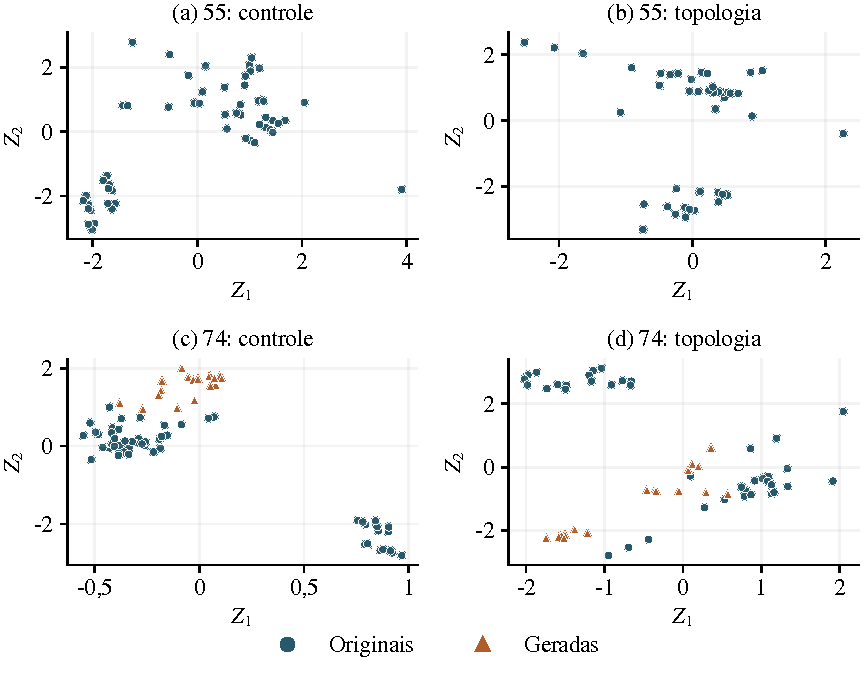
\includegraphics[width=\textwidth]{imgs/resultados/isa_quatro_modelos.pdf}
\begin{singlespace}
{\small Legenda: círculos indicam originais; triângulos, adições.
Escalas e orientações pertencem a cada ajuste; distâncias entre mapas
não são diretamente comparáveis.\par}
{\fonte{elaboração própria a partir das coordenadas dos modelos finais.}}
\end{singlespace}
\end{figure}

\FloatBarrier
\subsection{Diagnósticos internos e desbalanceamento dos rótulos}
\label{sec:res-isa-diagnosticos}

O rótulo bom, definido por \textit{gap} de até 10\%, não identifica o líder.
O IBS o recebeu em 70 das 74 instâncias, inclusive nas 19 adições, embora
liderasse somente duas delas. A solução sem recursos já satisfaz esse
limiar em 14 adições, incluindo as nove \textit{Huge}; assim, nem todas
ampliaram a dificuldade da classificação. Nos dois modelos de 74,
PYTHIA classificou todos os casos como bons para IBS: a acurácia simples
foi 94,59\%, mas a acurácia balanceada foi 50\%, pois nenhum dos quatro
negativos foi reconhecido.

A Tabela~\ref{tab:res-cv} apresenta o diagnóstico auxiliar repetido.
Nas 74 instâncias, a topologia elevou a média em 5,74 pontos percentuais
para ILS, 4,04 para LBBD e 5,12 para RS. CUTH e MIP perderam aproximadamente
0,73 e 0,31 ponto, e IBS permaneceu em 50,71\%. Os resultados nas 55
também variam entre métodos. Portanto, há contribuição descritiva e ganhos
internos específicos, sem melhora uniforme.

\begin{table}[!htbp]
\centering
\caption{Acurácia balanceada no diagnóstico auxiliar repetido.}
\label{tab:res-cv}
\begin{singlespace}
\normalsize
\setlength{\tabcolsep}{5pt}
\renewcommand{\arraystretch}{1.15}
\begin{tabular}{lrrrr}
\hline\hline
\textbf{Método} & \textbf{\shortstack{55\\controle}} & \textbf{\shortstack{55\\topologia}} & \textbf{\shortstack{74\\controle}} & \textbf{\shortstack{74\\topologia}} \\
\hline
IBS & $53{,}33\pm1{,}15$ & $53{,}33\pm1{,}15$ & $50{,}71\pm0{,}00$ & $50{,}71\pm0{,}00$ \\
MIP & $88{,}37\pm2{,}24$ & $89{,}80\pm2{,}58$ & $90{,}21\pm1{,}40$ & $89{,}90\pm2{,}67$ \\
CUTH & $84{,}69\pm6{,}29$ & $81{,}06\pm4{,}45$ & $91{,}72\pm1{,}15$ & $90{,}99\pm2{,}59$ \\
LBBD & $91{,}90\pm2{,}01$ & $93{,}14\pm1{,}81$ & $91{,}56\pm2{,}61$ & $95{,}60\pm0{,}92$ \\
ILS & $94{,}33\pm2{,}18$ & $94{,}55\pm1{,}33$ & $89{,}33\pm2{,}25$ & $95{,}07\pm1{,}09$ \\
RS & $91{,}94\pm8{,}08$ & $88{,}40\pm1{,}58$ & $87{,}92\pm1{,}64$ & $93{,}03\pm2{,}24$ \\
\hline\hline
\end{tabular}
\par\smallskip
{\small Nota: média em porcentagem $\pm$ desvio padrão amostral em pontos percentuais, em dez repetições de quatro partições. Coordenadas e hiperparâmetros foram obtidos globalmente; o procedimento não é aninhado nem externo.\par}
{\fonte{elaboração própria a partir dos dados experimentais.}}
\end{singlespace}
\end{table}


Como coordenadas e hiperparâmetros foram obtidos globalmente, esses valores
não estimam generalização externa do fluxo completo. O desvio padrão
resume dez repetições do particionamento; a seleção de atributos do SIFTED
usou uma única semente por ajuste, cuja estabilidade não é medida por essas
repetições. A leitura deve considerar
a diversidade da base, não apenas altas taxas de acerto, conforme a
perspectiva da ISA \cite{SmithMilesMunoz2023}.

Os \textit{footprints} mostram como essas predições se traduzem em regiões
de bom desempenho (Tabela~\ref{tab:res-footprints}). Nos quatro modelos,
o \textit{footprint} do IBS ocupa 100\% da área de referência construída pelo TRACE,
com densidade relativa e pureza iguais a um. Essa pureza é calculada a
partir das classes previstas, e não dos rótulos observados. Assim, a região
extensa acompanha a classificação generalizada como bom, mas não identifica
os casos em que o IBS ultrapassa o limiar de \textit{gap}. Para os demais
métodos, as regiões ocupam frações menores ou não chegam a ser construídas.
As diferenças entre mapas descrevem as respectivas geometrias e predições;
uma área maior não demonstra, por si só, maior competência observada.

\begin{table}[!htbp]
\centering
\caption{Área relativa dos footprints de bom desempenho nos quatro modelos.}
\label{tab:res-footprints}
\begin{singlespace}
\normalsize
\setlength{\tabcolsep}{7pt}
\renewcommand{\arraystretch}{1.12}
\begin{tabular}{lrrrr}
\hline\hline
\noalign{\vskip 3pt}
\textbf{Método} & \textbf{\shortstack{55\\controle}} & \textbf{\shortstack{55\\topologia}} & \textbf{\shortstack{74\\controle}} & \textbf{\shortstack{74\\topologia}} \\
\hline
IBS & 100,00 & 100,00 & 100,00 & 100,00 \\
MIP & 15,64 & 39,82 & 54,47 & 26,33 \\
CUTH & 0,00 & 0,00 & 4,38 & 11,07 \\
LBBD & 15,64 & 39,82 & 38,78 & 28,93 \\
ILS & 15,64 & 39,82 & 38,78 & 28,93 \\
RS & 0,00 & 0,00 & 4,38 & 6,47 \\
\hline\hline
\end{tabular}
\par\smallskip
{\small Nota: área do footprint dividida pela área de referência construída pelo TRACE no próprio mapa, em porcentagem. As regiões usam classes previstas, não rótulos observados. Zero indica ausência de região construída, não prova de incapacidade do método. As áreas absolutas de mapas diferentes não são diretamente comparáveis.\par}
{\fonte{elaboração própria a partir dos resultados dos quatro modelos.}}
\end{singlespace}
\end{table}


\section{Trajetórias de busca do IBS}\label{sec:res-stns}

\subsection{Instâncias clássicas no protocolo histórico}

As 160 execuções clássicas produziram 16 redes filtradas, com 10 a 37 nós.
LA0 apresentou 13 nós e fração compartilhada de 0,769, enquanto LB4 teve
31 nós, fração de 0,032 e oito assinaturas finais fora do conjunto de
melhor avaliação (Figura~\ref{fig:res-stn-classicas}). Esses casos contrastam
reutilização e dispersão das assinaturas. Suas forças de entrada limitadas,
0,6 e 0,1, descrevem frequências normalizadas, não probabilidades de sucesso.

O cruzamento das 16 redes com a PCA exploratória e os rótulos históricos
incluiu dez instâncias rotuladas como IBS, três como MIP e três como
LBBD ou ILS. As faixas de coordenadas desses grupos se sobrepunham nos
dois eixos da PCA. A fração compartilhada média foi 13,08\% no grupo IBS,
38,90\% no grupo MIP e 35,64\% nos demais; a média de estados finais não
melhores variou de 4,9 a 6,0 entre os grupos. Portanto, casos próximos
nessa representação podiam apresentar recorrências diferentes, e o rótulo
de melhor método não correspondia a um único perfil de trajetória do IBS.
Os dois grupos com três casos limitam a interpretação; esses rótulos
pertencem à exploração histórica, não à comparação final das 74 instâncias.

\begin{figure}[!htbp]
\centering
\caption{STNs históricas filtradas das instâncias LA0 e LB4.}
\label{fig:res-stn-classicas}
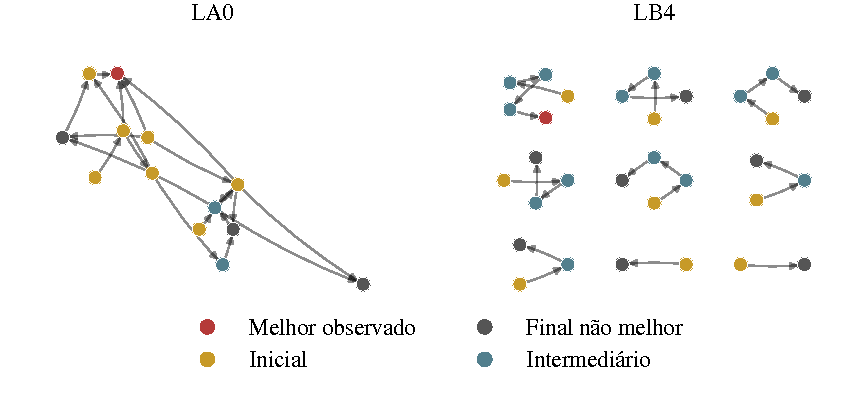
\includegraphics[width=\textwidth]{imgs/resultados/stns_classicas.pdf}
\begin{singlespace}
{\small Legenda: nós representam conjuntos protegidos e arestas conectam
assinaturas consecutivas na sequência filtrada. Melhor indica o menor
objetivo observado na rede; posições são apenas um arranjo gráfico.\par}
{\fonte{elaboração própria a partir dos registros históricos filtrados.}}
\end{singlespace}
\end{figure}

As redes complementam o objetivo final ao descrever o percurso
\cite{OchoaMalanBlum2021}. Entretanto, assinaturas sem instantes, orçamento
menor e limite de iterações impedem atribuir diferenças entre redes
históricas e adicionais isoladamente à expansão da coleção.

\subsection{Trajetórias suplementares com tempos decimais}

As 190 buscas adicionais, com tempos decimais preservados, produziram
36.593 registros e 2.682 estados distintos, contados por instância.
Houve 13.462 transições de piora, e todas as execuções apresentaram ao
menos uma. A última linha terminou pior que a incumbente em 123 buscas:
o desempenho final deve ser lido pela melhor solução preservada, não
pelo último estado da trajetória.

O filtro de não piora conservou 14.942 registros e 744 nós, mas pode ligar
assinaturas que não eram consecutivas no registro bruto. A rede filtrada
é uma sequência derivada; a bruta conserva os retornos a soluções piores.

O contraste por porte mostrou perfis diferentes nas redes brutas.
A única \textit{Small} apresentou 51 nós e Jaccard médio de 0,9412;
as três \textit{Medium}, de três a seis nós e Jaccard 1. Nas seis
\textit{Large}, os valores variaram de dois a 106 nós e Jaccard de
0,4500 a 1; nas nove \textit{Huge}, de 184 a 365 nós e Jaccard de
aproximadamente 0,0004 a 0,0774. Assim, as maiores redes das
\textit{Huge} acompanharam menor compartilhamento de estados entre
execuções. Como os limites de tempo também crescem com o porte, esse
contraste não isola o efeito do tamanho.

A Figura~\ref{fig:res-stn-suplementares} mostra
\textit{Large}-\texttt{00d0559e}, com dois estados e Jaccard 1, e
\textit{Huge}-\texttt{07952568}, com 365 estados e Jaccard 0,0173.
O primeiro caso atingiu objetivo 1.556 frente a BKV 1.515; o segundo,
6.355 frente a 5.942. Compartilhamento e diversidade não asseguram,
isoladamente, boa qualidade relativa.

\begin{figure}[!htbp]
\centering
\caption{Contraste entre duas STNs suplementares brutas do IBS.}
\label{fig:res-stn-suplementares}
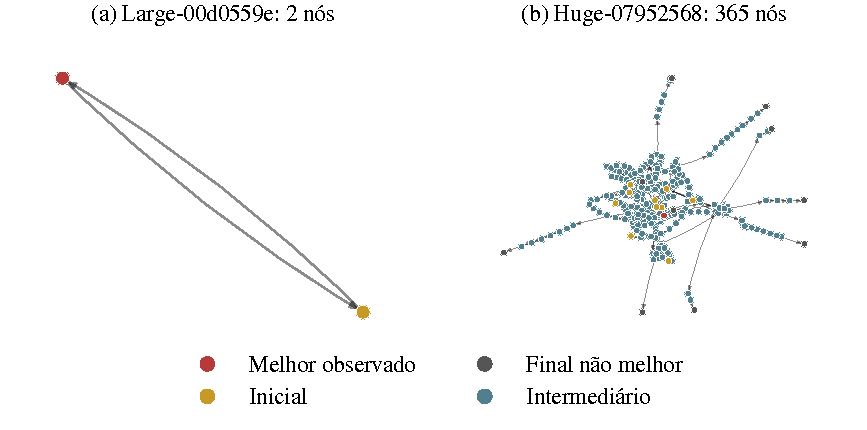
\includegraphics[width=\textwidth]{imgs/resultados/stns_suplementares.pdf}
\begin{singlespace}
{\small Legenda: dez execuções por instância. Nós são assinaturas
vértice--instante; arestas ligam estados consecutivos distintos.
As distâncias no desenho não representam diferenças de qualidade.\par}
{\fonte{elaboração própria a partir das redes brutas reconstruídas.}}
\end{singlespace}
\end{figure}

O tempo de parede excedeu o limite nominal nas 190 buscas, com excesso
relativo máximo de 5,28\%, pois o prazo é verificado entre chamadas
completas da busca em feixe. Ambiente e duração efetiva também diferiram
do histórico com tempos truncados, de modo que esse contraste não isola
o efeito da correção numérica. Nas \textit{Huge}, as STNs usam dez sementes,
enquanto as médias comparativas usam três.

\section{Relação entre instâncias, desempenho e trajetórias}\label{sec:res-integracao}

O cruzamento por identificador associou os descritores das STNs brutas
ao \textit{gap} médio IBS nas 19 adições (Tabela~\ref{tab:res-correlacoes}).
Nenhuma das cinco associações apresentou $p$ nominal inferior a 0,05.
Os descritores examinados não substituem diretamente a qualidade relativa,
sem que isso demonstre ausência de relações sob outros protocolos.
A interpretação considera a amostra dirigida e a diferença entre as
execuções usadas nas redes e no desempenho.

\begin{table}[!htbp]
\centering
\caption{Associação entre descritores das STNs brutas e \textit{gap} médio do IBS.}
\label{tab:res-correlacoes}
\begin{singlespace}
\normalsize
\setlength{\tabcolsep}{5pt}
\renewcommand{\arraystretch}{1.15}
\begin{tabular}{lrr}
\hline\hline
\textbf{Descritor} & \textbf{$\rho$ de Spearman} & \textbf{$p$ nominal} \\
\hline
Número de nós & 0,052 & 0,833 \\
Número de arestas & -0,133 & 0,586 \\
Finais distintos não melhores & 0,031 & 0,898 \\
Força de entrada sem teto & 0,328 & 0,171 \\
Jaccard médio & 0,004 & 0,989 \\
\hline\hline
\end{tabular}
\par\smallskip
{\small Nota: 19 instâncias geradas. Descritores das execuções complementares e \textit{gaps} do experimento comparativo, associados por instância. Correlações exploratórias, sem ajuste de multiplicidade nem interpretação causal.\par}
{\fonte{elaboração própria a partir dos dados experimentais.}}
\end{singlespace}
\end{table}


Em relação à hipótese da Seção~\ref{sec:pergunta-pesquisa}, a ampliação
revelou um regime favorável à CUTH, e as STNs distinguiram percursos não
descritos pelas médias finais. Na ISA, atributos topológicos foram
selecionados e sua inclusão alterou moderadamente a geometria dos mapas,
que mantiveram forte semelhança com o controle. A troca dos descritores
entre as coleções, sua associação parcial com o tamanho e os ganhos
preditivos heterogêneos não permitem concluir que a topologia ofereceu
informação independente dos atributos originais. Essa sustentação da
hipótese é descritiva: a mudança conjunta de porte, recursos e tempos
impede atribuir os contrastes exclusivamente à cobertura ou à topologia.
O estudo caracteriza a coleção avaliada, sem demonstrar causalidade,
generalização preditiva externa ou validade operacional em incêndios reais.
